\documentclass[a4paper]{article}

%Пакеты для математических символов:
\usepackage{amsmath} % американское математическое сообщество.
\usepackage{amssymb} % миллион разных значков и готический, ажурный шрифты.
\usepackage{amscd} % диаграммы, графики.
\usepackage{amsthm} % окружения теорем, определений и тд.
\usepackage{physics} % основные физические символы
%\usepackage{latexsym} % треугольники и пьяная стрелка.

%пакеты для шрифтов:
%\usepackage{euscript} % прописной шрифт с завитушками.
\usepackage{MnSymbol} % Значеки доказательства
\usepackage{verbatim} % улучшенный шрифт "пишущей машинки".
%\usepackage{array} % более удобные таблицы.
%\usepackage{multirow} % мультистолбцы в таблицах.
%\usepackage{longtable} % таблицы на несколько страниц.
%\usepackage{latexsym}

\usepackage{etoolbox}
\usepackage{slashbox} %Разделениени текста \backslashbox{}{}
\usepackage{collectbox} % Добавляет коробочки, можно складывать туда текст)


\usepackage{hyperref} % Ссылки как внешние так и внутренние
\hypersetup{
    colorlinks=true,
    linkcolor=black,
    filecolor=magenta,      
    urlcolor=cyan,
    pdftitle={Overleaf Example},
    pdfpagemode=FullScreen,
    }


%Пакеты для оформления:
\RequirePackage[center, medium]{titlesec}% Стиль секций и заголовков
%\usepackage[x11names]{xcolor} % 317 новых цветов для текста.
%\usepackage{multicol} % набор текста в несколько колонн.
\usepackage{graphicx} % расширенные возможности вставки стандартных картинок.
\usepackage{subcaption} % возможность вставлять картинки в строчку
%\usepackage{caption} % возможность подавить нумерацию у caption.
\usepackage{wrapfig} % вставка картинок и таблиц, обтекаемых текстом.
\usepackage{cancel} % значки для сокращения дробей, упрощения, стремления.
\usepackage{misccorr} % в заголовках появляется точка, но при ссылке на них ее нет.
%\usepackage{indentfirst} % отступ у первой строки раздела
%\usepackage{showkeys} % показывает label формул над их номером.
%\usepackage{fancyhdr} % удобное создание верхних и нижних колонтитулов.
%\usepackage{titlesec} % еще одно создание верхних и нижних колонтитулов

%Пакеты шрифтов, кодировок. НЕ МЕНЯТЬ РАСПОЛОЖЕНИЕ.
\usepackage[utf8]{inputenc} % кодировка символов.
%\usepackage{mathtext} % позволяет использовать русские буквы в формулах. НЕСОВМЕСТИМО С tempora.
\usepackage[T1, T2A]{fontenc} % кодировка шрифта.
\usepackage[english, russian]{babel} % доступные языки.

\usepackage{xcolor}
\definecolor{mycolor}{RGB}{244,228,215}

%Отступы и поля:
%размеры страницы А4 11.7x8.3in
\textwidth=7.3in % ширина текста
\textheight=10in % высота текста
\oddsidemargin=-0.5in % левый отступ(базовый 1дюйм + значение)
\topmargin=-0.5in % отступ сверху до колонтитула(базовый 1дюйм + значение)


%Сокращения
%Скобочки
\newcommand{\inrad}[1]{\left( #1 \right)}
\newcommand{\inner}[1]{\left( #1 \right)}
\newcommand{\infig}[1]{\left{ #1 \right}}
\newcommand{\insqr}[1]{\left[ #1 \right]}
\newcommand{\ave}[1]{\left\langle #1 \right\rangle}


%% Красивые <= и >=
\renewcommand{\geq}{\geqslant}
\renewcommand{\leq}{\leqslant}

%%Значек выполнятся
\newcommand{\per}{\hookrightarrow}

%%Векторная алгебра
\newcommand{\rot}{\text{rot}}
\renewcommand{\div}{\text{div}}
\renewcommand{\grad}{\text{grad}}


%% Более привычные греческие буквы
\renewcommand{\phi}{\varphi}
\renewcommand{\epsilon}{\varepsilon}
\newcommand{\eps}{\varepsilon}
\newcommand{\com}{\mathbb{C}}
\newcommand{\re}{\mathbb{R}}
\newcommand{\nat}{\mathbb{N}}
\newcommand{\stp}{$\filledmedtriangleleft$}
\newcommand{\enp}{$\filledmedsquare$}

\makeatletter
\newcommand{\sqbox}{%
    \collectbox{%
        \@tempdima=\dimexpr\width-\totalheight\relax
        \ifdim\@tempdima<\z@
            \fbox{\hbox{\hspace{-.5\@tempdima}\BOXCONTENT\hspace{-.5\@tempdima}}}%
        \else
            \ht\collectedbox=\dimexpr\ht\collectedbox+.5\@tempdima\relax
            \dp\collectedbox=\dimexpr\dp\collectedbox+.5\@tempdima\relax
            \fbox{\BOXCONTENT}%
        \fi
    }%
}
\makeatother
\newcommand{\mergelines}[2]{
\begin{tabular}{llp{.5\textwidth}}
#1 \\ #2
\end{tabular}
}
\newcommand\tab[1][0.51cm]{\hspace*{#1}}
\newcommand\difh[2]{\frac{\partial #1}{\partial #2}}
\newcommand{\messageforpeople}[1]{HSE Faculty of Physics \ \ HSE Faculty of Physics HSE Faculty of Physics \ \ HSE Faculty of Physics HSE Faculty of Physics \ \ HSE Faculty of Physics HSE Faculty of Physics \ \ HSE Faculty of Physics HSE Faculty of Physics \ \ HSE Faculty of Physics HSE Faculty of Physics \ \ HSE Faculty of Physics HSE Faculty of Physics \ \ HSE Faculty of Physics HSE Faculty of Physics \ \ HSE Faculty of Physics }


\numberwithin{equation}{section}

\begin{document}

\begin{flushright}
    Выполнил:

    Карибджанов Матвей
    
    Группа БФЗ211

    Тема:

    Поле излучения диполя
\end{flushright}
\tableofcontents
\newpagestyle{main}{
\setfootrule{0.4pt}
\setfoot{}{\thepage}{\sectiontitle}}
\pagestyle{main}
\pagecolor{mycolor}



\section{Постановка задачи}

Так так точные условия задачи не поставленны предлагаю рассмотреть 2 случая.

\subsection{Линейный осцилятор}
Первый рассеяние электромагнитной волны на линйном осциляторе, эту модель 
часто применяют для описания рассения на молекулах воздуха, с последующим 
выводом Реллевского рассеяния. 

Формульно зависимость между неподвижным ядром и оцилирующим элемнтом 
в квадратичном поле (квадратичное поле часто являтся результатом приближения), 
с "силой трения" силой линейно зафисящей от скрости элемента во избежании 
резонанса и бесконечного увелечнения амплитуды колебаний. В итоге получим:
\begin{equation}
    m\ddot r + mk \dot r + m\omega^2 r = f(r)
\end{equation}
Где $f(r)-$ некоторая вынуждающая сила.

В задачe в результате ускоренного движения диполь излучает 
электро-магнитные волны, котрые мы ищем.


\section{Излучение диполя}
\subsection{Уравнение Максвела}
В первую очередь надо вспомнить что для ЭМ (электромагнитный) волн 
ур. Максвелла преобразуются в:
\begin{gather}
    \begin{matrix}
        \rot E = -\cfrac{1}{c} \cfrac{\partial H}{\partial t} & div H = 0, \\
        \rot H = \cfrac{1}{c} \cfrac{\partial E}{\partial t} & div E = 0.
    \end{matrix}
\end{gather} 
По определению:
\begin{eqnarray}
    H &=& \rot A
\end{eqnarray} 
Учтя запаздывание потенциала, в следствии чего $A\inner{t - \cfrac{x}{c}}$:
\begin{gather}
    H = \insqr{\nabla, A} = -\cfrac{1}{c}\insqr{n, A'}.
\end{gather}
Зная что:
\begin{equation}
    A = \cfrac{1}{cR} \sum ev = \cfrac{1}{cR} \dot d.
\end{equation}
Так же не забываем про $E = \insqr{H, n}$, получим:
\begin{eqnarray}
    \begin{matrix}
        H = \cfrac{1}{c^2R}\insqr{\ddot d, n}, \\
        E = \cfrac{1}{c^2R}\insqr{\insqr{\ddot d, n}, n}.
    \end{matrix}
    \label{eq:2.5}
\end{eqnarray}
\begin{figure}[h]
    \centering
    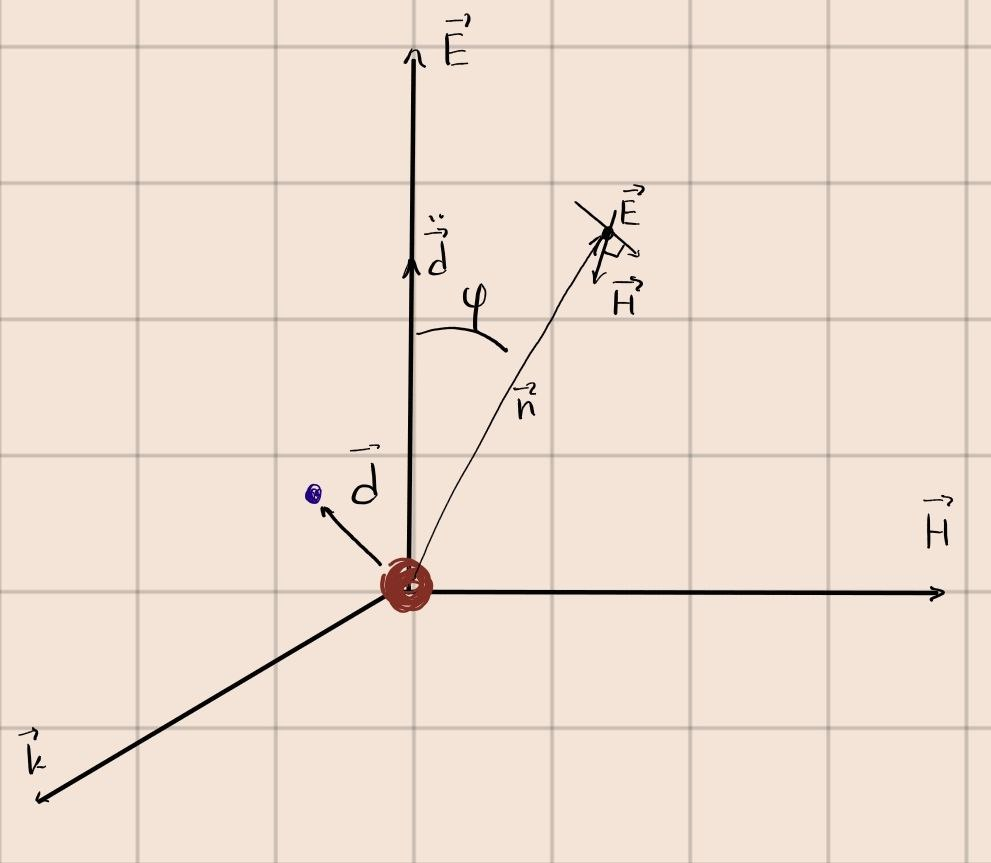
\includegraphics[trim={0 0 0 0},clip,width=\textwidth]{sh.jpg}
    \label{pict}
\end{figure}

\subsection{Вектор пойнтинга}
Учитывая ортогональность векторов $H$ и $E$, также то что в 
монохроматической волне $\abs{H} = \abs{E}$, то вектор Пойнтинга
\begin{equation}
    S = \cfrac{cH^2}{4\pi}n.
\end{equation}
От сюда получим 
\begin{equation}
    d\mathfrak{I} = \cfrac{cH^2}{4\pi}R^2do
    \label{eq:2.7}
\end{equation}

\subsection{Частотное пространство}

Часто удобно работаь в спектральном разложении поэтому посмотрим 
на зависимомти в фурье образа. Напрямую из переобразования формул 
\ref{eq:2.5} получим:
\begin{gather}
    \begin{matrix}
        H_\omega = i \insqr{k, A_\omega},\\
        E_\omega = \cfrac{ic}{\omega} \insqr{k, \insqr{k, A_\omega}},
    \end{matrix}
\end{gather}
Воспользовавшись формулой 
\begin{equation}
    \int_\re f^2 dt = \int_\re \abs{f_\omega}^2 \cfrac{d\omega}{2\pi} 
    = 2\int_{\re_+} \abs{f_\omega}^2 \cfrac{d\omega}{2\pi} 
\end{equation}
Заметив что от в \ref{eq:2.7}  зависит от $t$ только посредстаом $H$ 
получим:
\begin{equation}
    d\mathfrak{I} = \cfrac{c}{2\pi} \abs{H}^2R^2do
    \label{eq:if}
\end{equation}



\section{Решение для линейноного осцилятора}
\subsection{Приближения и уточнение формулировки}

Во первых вспомнм что:
\begin{equation}
    p  = \cfrac{mv}{\sqrt{1 - \cfrac{v^2}{c^2}}}.
\end{equation}
В не релятивистком случае уравненнеие сильно упрощается:
\begin{equation}
    p \approx mv,
\end{equation}
поэтому предлагаю решать в приближении $v/c \ll 1$.
Тогда известное нам уравнение:
\begin{equation}
    \cfrac{dp}{dt} = e  E + \cfrac{e}{c} \insqr{ v,  H},
\end{equation}
выродится в: 
\begin{equation}
    m\cfrac{dv}{dt} = e  E.
\end{equation}

Будем рассматривать падение на диполь монохроматической волны. 
Пока что мне не нужна точная формула, а только одно очень 
удобное свойство:
\begin{equation}
    \mathfrak F\insqr{ E (t)}(\omega) =  E (\omega).
\end{equation}

\subsection{Диф. уравнение}
 
Запишем наше уравнение:
\begin{equation}
    m \ddot r + mk\dot r + m\omega_0^2r = e E(t).
\end{equation}
Как уже ясно я предлагаю использовать преобразование фурье для решения:
\begin{equation}
    -\omega^2 r - i\omega kr + \omega_0^2r = \cfrac{e}{m} E(\omega).
\end{equation}
Вспомним что в излучение диполя основной вклад дает компонента $\ddot d$,
А так как так как центральный заряд не подвижен и закреплен в начале СО 
то $ d = e r \implies \ddot{{{d}}} = e\ddot{{r}}$. Тогда 
нам нужно искать:
\begin{equation}
    r = \cfrac{eE(\omega)}{m\inner{\omega_0^2 - i\omega k - \omega^2 }}.
\end{equation}
\begin{equation}
    \mathfrak F \insqr{\ddot d}(\omega)= -e\omega^2 r = 
    -\cfrac{e\omega^2E(\omega)}{m\inner{\omega_0^2 - i\omega k 
    - \omega^2 }}.
    \label{eq:ddot_d}
\end{equation}

Получим распределение полей:
\begin{equation}
    E = \cfrac{e}{mc^2R}\insqr{\int_\re
    \cfrac{\omega^2E_\omega}{\inner{\omega_0^2 - i\omega k - \omega^2 }}\exp{-it\omega}\cfrac{d\omega}{2\pi}, n},
    \label{eq:fild}
\end{equation}
\begin{equation}
    H = \insqr{E, n}.
\end{equation}

\subsection{Распределение интенсивности}

Пользуясь формулой \ref{eq:if} получим:
\begin{equation}
    d\mathfrak{I} = \cfrac{1}{4\pi c^3}\insqr{\ddot{d}, n}^2do
    = \cfrac{1}{4\pi c^3}\ddot d^2_\omega \sin^2\phi do.
\end{equation}
Подставляем решение \ref{eq:ddot_d}:
\begin{equation}
    d\mathfrak{I} = \cfrac{1}{4\pi c^3} \abs{\cfrac{eE(\omega)}{m\inner{\omega_0^2 
    - i\omega k - \omega^2 }}}^2 \sin^2\phi do.
\end{equation}
Проинтегрируем по всем углам, использовав соотношение $do = 2 \pi \sin{\phi} d\phi$:
\begin{equation}
    \mathfrak{I} = \cfrac{2}{3c^3} \ddot{d}^2_\omega.
\end{equation}

\begin{figure}[h]
    \centering
    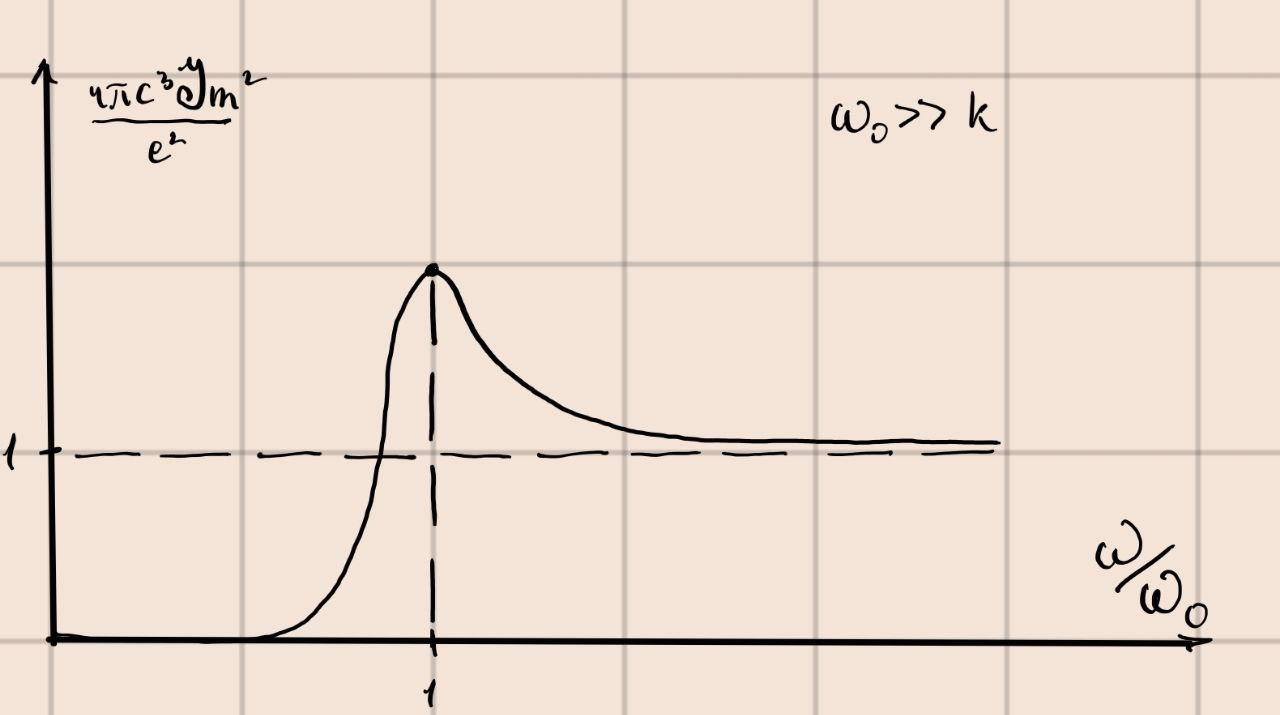
\includegraphics[trim={0 0 0 0},clip,width=0.5\textwidth]{omega.jpg}
    \label{pict}
\end{figure}
\begin{figure}[h]
    \centering
    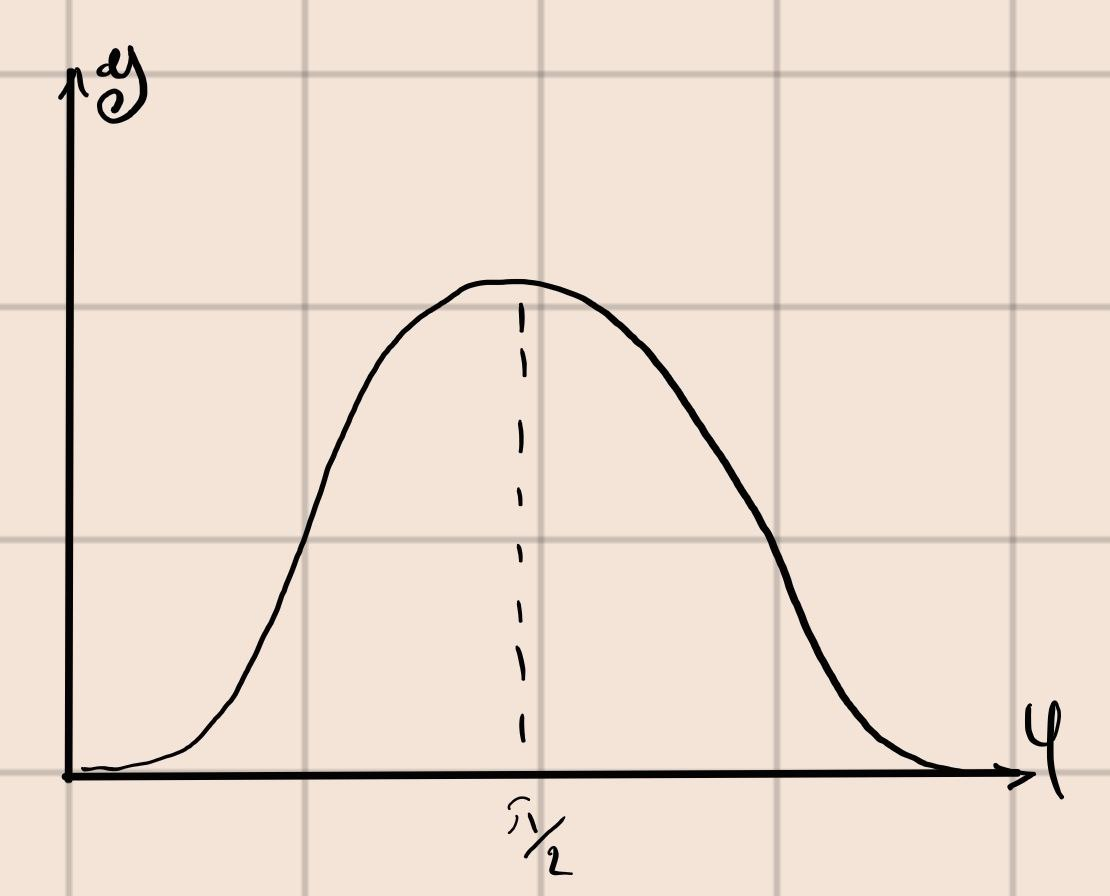
\includegraphics[trim={0 0 0 0},clip,width=0.5\textwidth]{phi.jpg}
    \label{pict}
\end{figure}


\section{Вывод}

Как мы видим для знания поля нужна информация о параметрах диполя. 
Например для велечины поля по формуле \ref{eq:fild}. Для решении 
не использовались вектора Герца, было очень удобно пользоваться 
формализмом векоторного потенциала.




\end{document}